\section{Instrumenteringsforstærker}\label{sec:summa}
For at få en retning ud af spolesignalerne, anvendes instrumenteringsforstærkeren AD623. Denne IC har to input pins - en til hver af modtagerspolerne.
Netop instrumenteringsforstærkeren AD623, er valgt frem for andre operationsforstærker typer, af grundlæggende årsager; for det første er det en differensforstærker, hvilket betyder at den forstærker differensspændingen som fås ved $V_{udgangssignal} = V_{in_1} - V_{in_2}$. Da instrumenteringsforstærkeren internt består af flere operationsforstærkere, har den en høj indgangsimpedans, og samtadig kan forstærkningen styres med blot en gainmodstand, hvilket sparer plads på print boardet.

\begin{figure}[h!]
	\centering
	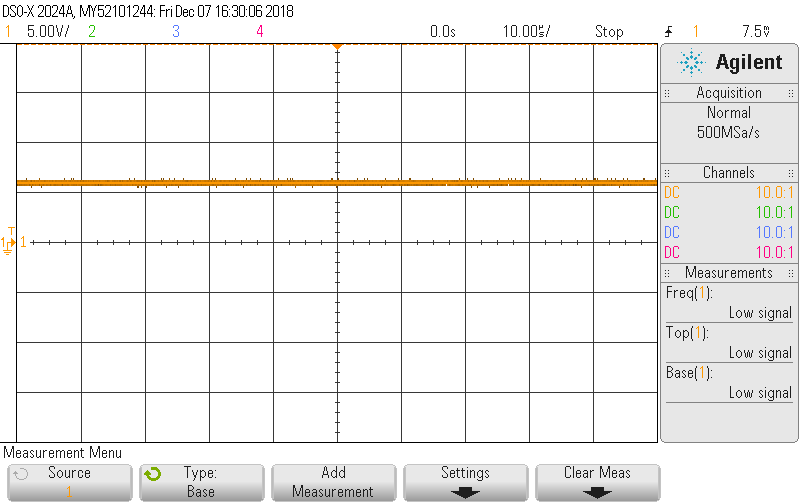
\includegraphics[width=1\textwidth]{billeder/instr_png.png}
	\caption{Billedet her viser outputtet fra instrumenteringsforstærkeren, hvor spolerne er i en tilfældig position.}
	\label{fig:filter_out}
\end{figure}

\subsection{Design}
\begin{wrapfigure}{r}{0.5\textwidth}
	\centering
	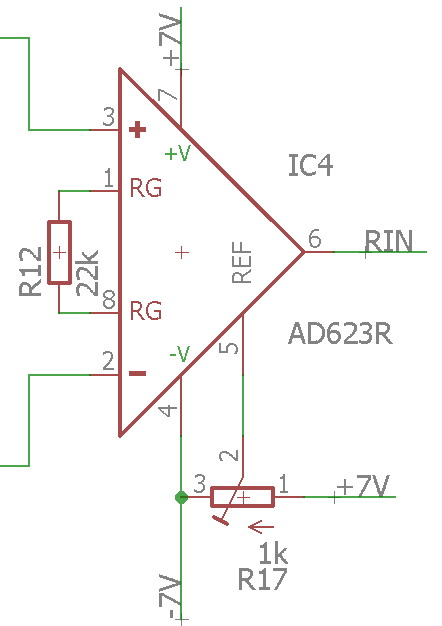
\includegraphics[width=0.48\textwidth]{billeder/instrumentation_amplifier.png}
	\caption{Diagram over instrumenteringsforstærkeren.}
	\label{fig:instrumentation_amplifier}
\end{wrapfigure}
Det samlede kredsløb for instrumenteringsforstærkeren består af en AD623, en gain modstand, samt et potentiometer. Dertil er der påsat to afkoblingskondensatorer. Kredsen forsynes med $\pm 7 \si{\volt}$, da det er max output fra batterierne. 

\subsection{Beregninger}
Da indgangssignalerne til instrumenteringsforstærkeren er meget lave, anvendes en gainmodstand for at forstærke signalet.

Der tilstræbes en forstærkning på 4 - 5 gange. Forstærkningen udregnes med ligningen fra fra databladet \cite[side 11]{AD623}.
\begin{align}
	R_G & = \frac{100 \si{\kilo\ohm}}{G-1}
\end{align}
hvor en gainmodstand på $R_G = 22 \si{\kilo\ohm}$ giver en forstærkning på \num{4.5}.